\documentclass[10pt]{article}
 
\usepackage[margin=1in]{geometry} 
\usepackage{amsmath,amsthm,amssymb, graphicx, multicol, array, multirow, subfig}
\usepackage{enumitem}
\usepackage{hyperref}
\usepackage[table]{xcolor}
\usepackage{ctable}
 
\newcommand{\N}{\mathbb{N}}
\newcommand{\Z}{\mathbb{Z}}
 
\newenvironment{problem}[2][]{\begin{trivlist}
\item[\hskip \labelsep {\bfseries #1}\hskip \labelsep {\bfseries #2.}]}{\end{trivlist}}

\date{Due: Friday, Dec 16, 2022 10pm PT}

\begin{document}
 
\title{Fall 2022: Final Exam}
\author{
CS 181AG: Network Algorithmics}
\maketitle

Under the Honor Code, this document is not to be shared with anyone.

\begin{itemize}

\item The exam will be made available on Gradescope on Saturday, Dec 10th, 2022 at 8am PT. It will be due Friday, Dec 16th, 2022 at 10pm PT through Gradescope. Please ensure you leave enough time for the submission process as there is no late allowance for the exam.

\item During the exam, you will have access to your course materials: lecture slides, videos, assignments, textbook, midterm, and photos of board work from class. You may not access ANY other resources, including other websites, textbooks, or people.

\item Though the exam will be untimed, you will be expected to take it in one sitting. However, you may
take short breaks as needed, e.g. to rest your eyes, grab a snack, change background music, or use the
restroom. Long breaks that include a substantial context switch (e.g. working on another assignment,
having an extended conversation with someone, leaving the area where you’re taking the exam) are
not allowed.

\item You should not contact anyone, including Prof. Arthi, during the exam period. If you have unresolved
questions about the exam, you may include a note about your question and the assumption you made
to address it. Such notes will be taken into consideration when grading the exam.

\item Your exam will be submitted as a PDF. You may answer questions, fill in tables, etc by handwriting, using LaTeX, or any other method you use for your assignments. As with all assignments, you will need to mark the answer regions in Gradescope.

\item The exam will be scored out of 100 points over 7 questions, divided by topic.

\end{itemize}

\newpage
\begin{problem}{1: Link-State Infinite Loops}
\item In class, we discussed two types of routing protocols, distance-vector and link-state. Assume that the network below is running a link-state protocol, and each node has calculated its shortest path to each other node and is forwarding packets accordingly.

\begin{figure}[h]
    \centering
    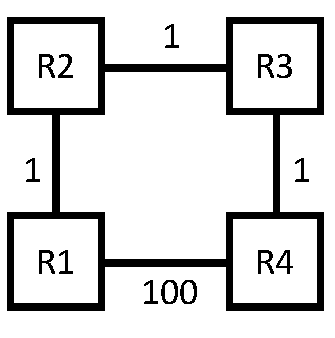
\includegraphics[scale=0.6]{figures/link_state.pdf}
    \label{fig:link_state}
\end{figure}

\begin{enumerate}
    \item Describe a series of events (e.g., a link goes down, a node recalculates its routes) that would lead to a packet looping infinitely between R2 and R3.
    \item Describe a series of events (e.g., a link goes down, a node recalculates its routes) that would lead to a packet looping infinitely between R1 and R2.
    \item True or False: link-state protocols require less memory than distance-vector. Explain your reasoning. 
\end{enumerate}

\end{problem}

\subsection*{Answer 1:}
In this problem, I am assuming that we are talking about the temporary loops that can occur under Link-State protocols.
\begin{enumerate}
  \item A series of events that would lead to a packet looping infinitely between R2 and R3 would be if the path between R4 and R3 were broken and if R3 were to find out immediately and were to recalculate its paths immediately after but then sends a packet before sending its updated table to the other nodes. This would cause a temporary infinite loop if R3 or R2 were to decide to send a packet to R4, as R3, knowing about the break, would find that R2 would be its best route to R4, but that since R2 has not updated its table, it thinks that its best route is through R3, leading to a temporary infinite loop.
  \item A series of events that would lead to a packet looping infinitely between R1 and R2 would be if we were to break the connection between R2 and R3 and then, finding out abou this immediately, R2 recalculates its paths and then immediately sends a packet to R1 before updating R1 about the changes to its topology. This would cause an infinte loop between R1 and R2 that would persist until R2 updates R1 with its new topology since R2 will try to go through R1, but R1 will try to go through its old topology link of R2 since 2 $<$ 100.
  \item This is false. In link-state protocol, each nodes stores the entire network toplogy where as in distance-vector does not require the storage of all edges between nodes.
\end{enumerate}

\begin{problem}{2: Longest Matching Prefix Caching}
Your friend proposes a scheme to find the longest-matching-prefix using caching. This is their plan: keep a small set of prefixes in a cache. When a packet arrives, run a longest-matching-prefix search within the cache. If a prefix is found, return the next hop corresponding to the prefix. If no prefix is found, run a longest-matching-prefix search across the rest of the database, return the next hop corresponding to the longest matching prefix, and insert the longest matching prefix into the cache. \\\\
You realize that your friend's plan has a fundamental flaw. Explain the flaw and give an example where your friend's scheme would return an incorrect answer.
\end{problem}

\subsection*{Answer 2:}
The fundamental flaw with the solution is that this solution assumes that if we find a prefix in the cache, then it follows that we have found the longest matching prefix. However, this may not be true. Consider that we could possibly have a prefix e.g. 01* in our cache from one of our earlier lookups and that at the same time, we had 01110* in our database. Then it would follow that if we were to lookup the string 011101010 we would have a longer matching prefix in our database, but under this scheme, since we found \textbf{a} matching prefix in our cache of 01*, then we would use the next hop corresponding to the said cached prefix without even considering the database to find a longer matching prefix, thus defeating the point of the algorithm as we would not find the "longest matching prefix".
\begin{problem}{3: Switching}
Consider a router with the following sets of input and output ports. The queues of packets are shown next to each input. As in class, the number denotes which output queue the packet is intended for, and the head of the queue is at the right (i.e., the head of A's queue is 1).

\begin{figure}[h]
    \centering
    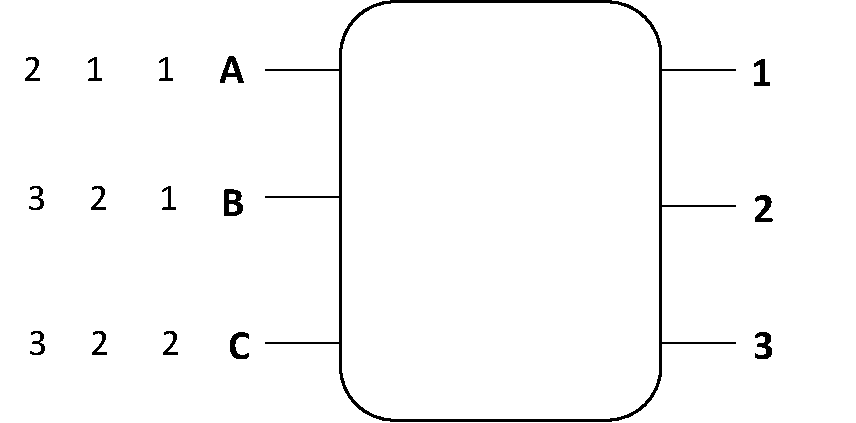
\includegraphics[scale=0.6]{figures/islip.pdf}
    \label{fig:islip}
\end{figure}

\begin{enumerate}
    \item The router is using the \textbf{iSLIP} algorithm. Assume that the algorithm is just starting, so all grant and accept pointers start at their initial positions. Which input ports send to which output ports in Round 1? For each matched pair, specify in which iteration they were matched. 
    \item Where are the accept pointers for input ports A, B, and C after Round 1? Where are the grant pointers for output ports 1, 2, and 3 after Round 1?
\end{enumerate}
\end{problem}

\subsection*{Answer 3:}
\begin{enumerate}
  \item Using the \textbf{iSLIP} algorithm set to initial positions (where all \textbf{A, B, C} pointers point to 1 and \textbf{1,2,3} point to \textbf{A}), we have \textbf{1} and \textbf{A} matching in iteration 1, \textbf{3} and \textbf{B} matching in iteration 1, and \textbf{2} and \textbf{C} matching in iteration 2.
  \item After round 1, the accept pointer for input port A points at 2, the accept pointer for input port B points at 1, and the accept pointer for input port C also points at 1. After round 1, the grant pointer for output port 1 is pointed at B, the grant pointer for output port 2 still points at A, and the grant pointer for output 3 points at C.
\end{enumerate}
\begin{problem}{4: TCP Connection}
Node 1 wants to send a 5 byte message (which can all be sent in one packet) over TCP to Node 2 at port 25. They currently do not have a TCP connection open. Node 1 is behind a router which implements Network Address Translation, with the public/private IP addresses shown in Figure \ref{fig:tcp-setup}, and Node 2 is out of the network and directly connected to the router, with its IP address also shown in Figure \ref{fig:tcp-setup}.

\begin{figure*}[ht]
\centering

\subfloat[]{%
  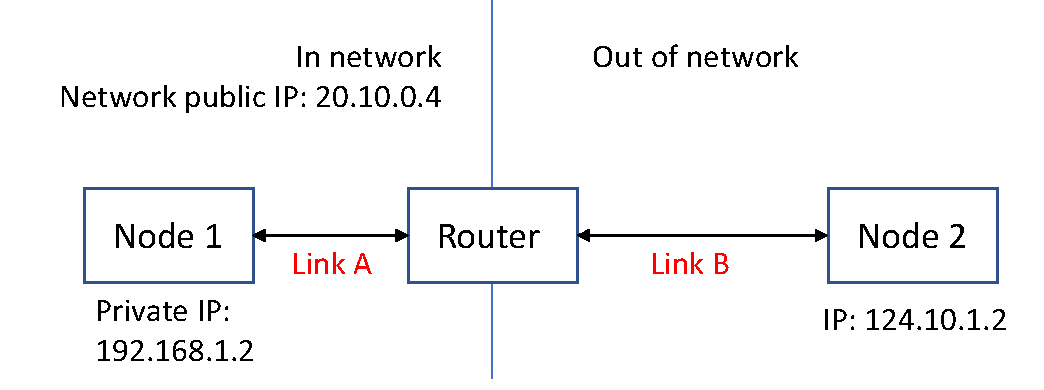
\includegraphics[scale=0.6]{figures/tcp_connection.pdf}%
  \label{fig:tcp-setup}%
}\qquad
\subfloat[]{%
  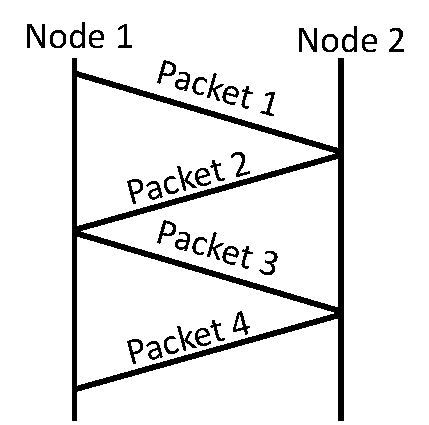
\includegraphics[scale=0.5]{figures/tcp_communication.pdf}%
  \label{fig:tcp-communication}%
}
\label{fig:tcp}
\caption{Topology (a) and first four packets (b) for Nodes 1 and 2}

\end{figure*}

Figure \ref{fig:tcp-communication} shows the first four packets sent in this exchange. Packet 4 acknowledges that Node 2 received Packet 3, the 5-byte message.

Fill out the table below showing a subset of the packet header for each of the four packets. For each packet, there are two rows, one for each link: between Node 1 and the router (Link A), and between the router and Node 2 (Link B). The links are shown in the order the packet traverses them (Packet 1 is sent from Node 1 across Link A to the router, and then from the router across Link B to Node 2, hence Link A is listed before Link B). For columns 3-8, write the IP or number. For the last 2 columns, put an x if the corresponding flag is set. The first row is filled out for you as an example.
 \\
Notes: 
\begin{enumerate}
    \item You may leave some entries blank if they don't correspond to meaningful information.
    \item Please make up a (valid) port number where applicable, but remember to be consistent about your use of this number in subsequent communications.
\end{enumerate}

\setlength\extrarowheight{8pt}
\begin{table}[ht]
    \begin{center}
    \begin{tabular}{|c|c|c|c|c|c|c|c|c|c|}
    	\hline
    	  Packet & Link & Src IP & Dst IP & Src Port & Dst Port & Seq Num & Ack Num & SYN & ACK \\
    	\hline
    	Packet 1 & Link A & 192.168.1.2 & 124.10.1.2 & 17500 & 25 & 0 & & x &\\
    	\hline
    	Packet 1 & Link B & 20.10.0.4 & 124.10.1.2 & 1502 & 25 & 0 & & x &\\
    	\specialrule{.3em}{.2em}{.2em}
             Packet 2 & Link B & 124.10.1.2 & 20.10.10.4 & 25 & 1502 & 0 & 1 & x &x\\
    	\hline
    	  Packet 2 &  Link A & 124.10.1.2 & 192.168.1.2 & 25 & 17500 & 0 &1 & x& x\\
    	\specialrule{.3em}{.2em}{.2em}
            Packet 3 &  Link A & 192.168.1.2 & 124.10.1.2 & 17500 & 25 & 1 & 1 & & x\\
    	\hline
    	  Packet 3 & Link B & 20.10.0.4 & 124.10.1.2 & 1502 & 25 & 1 &1 & &x\\
    	\specialrule{.3em}{.2em}{.2em}
            Packet 4 & Link B & 124.10.1.2& 20.10.04& 25& 1502&2 & 6 & &x\\
    	\hline
    	  Packet 4 &  Link A & 124.10.1.2 & 192.168.1.2& 25& 17500&2 & 6 & &x\\
    	\specialrule{.3em}{.2em}{.2em}
    	
    \end{tabular}
    \end{center}
    \end{table}


\end{problem}
\newpage
\begin{problem}{5: TCP Congestion Control}
Your computer and your friend's computer are communicating using a TCP connection. After the 3-way handshake, the window size is 1. Your computer sends Packet 1 to your friend's computer, and its receipt is acknowledged. The window size is now 2. Then, your computer sends Packets 2 and 3 to your friend's computer, and those are acknowledged as well. The window size is now 4. Then, your computer sends Packets 5, 6, 7, and 8, and all are successfully received by your friend's computer \textbf{except Packet 5}.
\begin{enumerate}
    \item Assume your friend's computer sends an ack packet in response to receiving each packet: 6, 7, and 8, so 3 packets in total. What is the ack number of each of these packets?
    \item If we observe all the routers on the route between the two computers, we see that all of them have room in their input queues and output queues, i.e., none are completely full. Describe why a non-full router could still drop Packet 5.
    \item Based on the ack numbers of Packets 6, 7, and 8 (which you filled out in part 1), your computer realizes there there is congestion and resends Packet 5, which this time successfully reaches and is acknowledged. Which packets can be sent next before receiving any more acks? (Note: resending Packet 5 does not affect the window size). Explain your response.
    \item Let's say the packets sent in your response to part 3 were successfully sent and acknowledged. Which packets can be sent next before receiving any more acks? Explain your response.
\end{enumerate}
\end{problem}
\subsection*{Answer 5:}
The wording of this question is throwing me a bit off. Wouldn't we send Packet 4 before Packets 5,6,7,8? Since our window size is 4, wouldn't we only be able to send packet 8 if we knew that 4 was receieved? I am operating under the assumption that Packet 4 was sent and acknowledged.z
\begin{enumerate}
  \item The ack number of packet 6 is 4. The ack number of packet 7 is 4. The ack number of packet 8 is 4.
  \item There are a nmber of different algorithms that can be used by the routers that would result in the dropping of packets even if the router is not full. For example, if RED was being implemented within a router and that router had an output queue that was greater than the specified threshold, then we have a non-zero probability of dropping the packet.
  \item After resending Packet 5, we recieve an ack number of 8 since at the point, the friends computer will have recieved all of the packets and would send an ack number of 8 (all before and including 8 have been recieved). Thus, we can send Packets 9, 10 since resending Packet 5 does not affect our window size, but that since we encountered duplicate ACKs, it follows that our window size is halved, which, as it was 4 before, it is now 2.
  \item Assuming that packets sent in the prior part arrived and were acknowledged successfully, then it would follow that we could send the Packets 11, 12, 13, and 14, since we are now sending in a new transmission round, and, assuming that we had a threshold intially of 16, we would have a threshold of 8 after the duplicate acks are detected, and as we are below that threshold, we would have exponential growth ($2 \to 4$).
\end{enumerate}
\newpage
\begin{problem}{6: Balancing Flow}
Consider a single output queue at a router that contains 3 different flows. The packets that need to be sent for each flow are shown below, each labelled with the number of Mb in the packet. As in class, the front of the queue is at the right.

We want each flow to send at an long-term rate of 4Mbps with a burst size of no more than 6Mb. Therefore, we use deficit round robin (where 1 token = 1Mb). We give each flow a bucket that can hold at most 6 tokens, and we give each flow 4 tokens at the beginning of each round.

\begin{figure}[h]
    \centering
    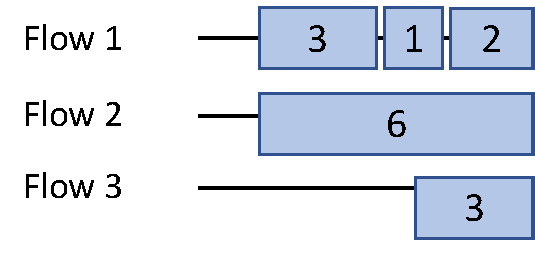
\includegraphics[scale=0.8]{figures/drr.pdf}
    \label{fig:bin_search}
\end{figure}
\begin{enumerate}
    \item Which packets get sent in the first round of the round robin and in what order? Denote the packets using the [flow ID]-[size] format, e.g., 1-2 is a packet from Flow 1 with size 2.
    \item Before the second round of the round robin, after you adjust each flow’s token bucket (so they’re now ready to send again), how many tokens are in each flow’s bucket? Assume that no additional packets arrive.
    \item Suppose we want to adjust our per-flow long-term rates so that the total rate for the output queue stays the same (12Mbps), but Flow 1 now gets 50\% of that total rate, while Flows 2 and 3 split the remainder. Flow 1 also now gets a max burst size of 10Mb, and Flows 2 and 3 should still have a max burst size of 6Mb. What is the size of each flow's bucket? How many tokens does each flow get at the beginning of each round?
\end{enumerate}
\end{problem}
\subsection*{Answer 6:}
\begin{enumerate}
  \item The packets that get sent in the first round of the round robin are 1-2, 1-1, 3-3.
  \item After adjusting each flow's token bucket (assuming that this means removing the costs and then adding in the 4 tokens into the bucket), Flow 1 has 5 tokens, Flow 2 has 8 tokens, and Flow 3 has 0 tokens.
  \item The size of Flow 1's bucket is 10 tokens and Flows 2 and 3 both have buckets of size 6 tokens. At the beginning of rounds, Flow1 gets 6 tokens and Flows 2 and 3 both get 3 tokens.
\end{enumerate}


\begin{problem}{7: DNS lookups}
Suppose your device wants to send an HTTP request to the HMC server and get back a response (each 1 packet). However, all DNS caches are initially empty (including your device’s DNS resolver's cache). Each trip between device/server and server/server takes exactly 5ms, so each round trip takes 10ms.

\begin{enumerate}
    \item How long does it take for your device to get the IP address of the HMC server? 
    \item Once your device has the IP address of the HMC server, how long does it take to get the HTTP response?
\end{enumerate}

There may be multiple correct answers - any are acceptable. Hint: remember which protocol is used for each step. Show your work!
    
\end{problem}
\subsection*{Answer 7:}
\begin{enumerate}
  \item It takes 30 ms to get the IP address of the HMC server. After recognizing that our cache is empty, we go to the DNS resolver (5 ms), then from there, assuming that the IP address is not in the resolver cache, then we go to the Root name server to get the IP of our .edu server which takes 10ms to get, then we get the IP of our hmc.edu server from our Top Level Domain Server which takes another 10 ms. Then, this IP is returned to our device from the DNS resolver in 5ms giving us a total of 30 ms.
  \item Once the device has the IP address of the HMC server, it takes 10 ms to get the HTTP response since we go directly to the server, hmc.edu, and request the HTTP file from that server in giving them the IP address. Thus, we should have 1 device/server interaction.
\end{enumerate}

\begin{problem}{8}
How long did this exam take you? How would you rate the difficulty on a scale from 1-10 (10 being the hardest)? Feel free to share any other thoughts on the final, or your preparation, or this class. \\\\
This exam took me $\approx 3$ hours. I would rate the difficulty at about a 7 since there were some instances where I felt like I had to make some assumptions and where I felt challenged and had to think critically about what I was doing. I did not feel blind sided by anything on the final though which I appreciate, I felt as though I had seen every topic on the exam before, though some questions seemed to be in a new manner which was cool to think about and to synthesize. The class was incredibly interesting and I really enjoyed my time in it as well as the material. I feel as though I learned a lot this semester and I really appreciate your work to be flexible with the class and to faciliate a deep understanding of the material. I hope you have a great break! Thank you Prof. Arthi!\\\\
Congratulations on finishing all requirements for CS181AG! I hope you learned a lot this semester and that you have a restful holiday season :) 



\end{problem}
\end{document}

